% 2015_hunan_liberal_q18_fig1: 直三棱柱 ABC-A1B1C1, E在BC中点, F在CC1中点
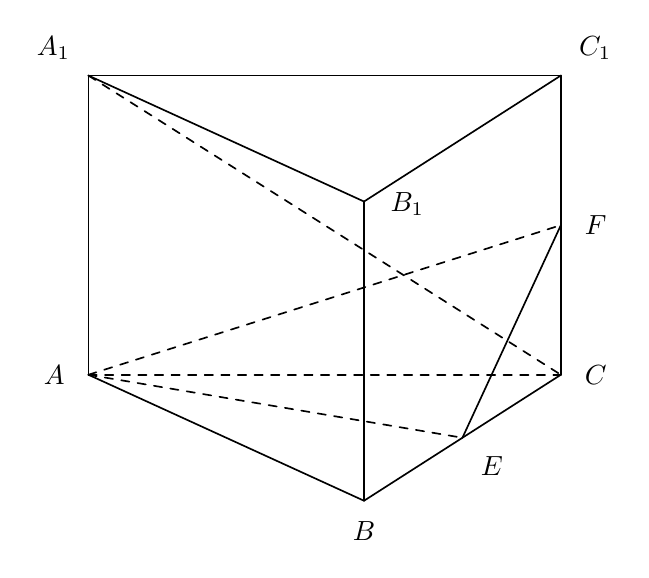
\begin{tikzpicture}[line width=0.6pt, line join=round, line cap=round, font=\normalsize]
\coordinate (A1) at (0,4.2);
\coordinate (C1) at (6,4.2);
\coordinate (B1) at (3.5000000000,2.6000000000);
\coordinate (A) at (0,0.4);
\coordinate (C) at (6,0.4);
\coordinate (B) at (3.5,-1.2);
\coordinate (E) at (4.75,-0.4);
\coordinate (F) at (6,2.3);
% 棱柱可见棱(实线)
\draw (A1) -- (C1);
\draw (A1) -- (B1);
\draw (B1) -- (C1);
\draw (A1) -- (A);
\draw (B1) -- (B);
\draw (C1) -- (C);
\draw (A) -- (B);
\draw (B) -- (E);
\draw (E) -- (C);
\draw (E) -- (F);

% 内部/遮挡棱(虚线)
\draw[dashed] (A) -- (C);
\draw[dashed] (A) -- (E);
\draw[dashed] (A) -- (F);
\draw[dashed] (A1) -- (C);
% 标签(避碰外置)
\node[above left, xshift=-3pt, yshift=2pt] at (A1) {$A_{1}$};
\node[above right, xshift=3pt, yshift=2pt] at (C1) {$C_{1}$};
\node[right, xshift=6pt,yshift=-1pt] at (B1) {$B_{1}$};
\node[left, xshift=-5pt] at (A) {$A$};
\node[right, xshift=5pt] at (C) {$C$};
\node[below, yshift=-4pt] at (B) {$B$};
\node[below right, xshift=3pt, yshift=-3pt] at (E) {$E$};
\node[right, xshift=5pt] at (F) {$F$};
\end{tikzpicture}
